\chapter{Alkenes and Alkynes: Electrophilic Additions}\label{ch:b1:electrophilic-additions}

Shake an alkene with orange bromine water and the colour vanishes in
seconds: the oldest test for a carbon--carbon double bond. Behind it is a
mechanism. The $\pi$ electrons of the double bond, held less tightly than
the $\sigma$ electrons and exposed above and below the plane of the
molecule, attack an electron-poor reagent; the cation formed then
captures a \omterm{def:b1:electronic-effects:nucleophile}{nucleophile}. The same two steps add hydrogen halides, water
and halogens to alkenes, decide which carbon receives which part of the
reagent, and fix the stereochemistry of the product. This chapter
develops them, with the rule a nineteenth-century chemist drew from
observation and the \omterm{def:b1:electronic-effects:intermediates}{carbocation} that explains it.

\begin{recall}
\omterm{def:b1:electronic-effects:intermediates}{Carbocations}, their stability and \omterm{def:b1:electronic-effects:curly-arrow}{curly arrows} (\cref{ch:b1:electronic-effects});
the Hammond postulate (\cref{prop:b1:elementary-steps:hammond}); $Z$/$E$
descriptors, \cip{R}/\cip{S}, \omterm{def:b1:stereochemistry-in-depth:enantiomers}{meso compounds} and \omterm{def:b1:stereochemistry-in-depth:enantiomers}{racemic mixtures}
(\cref{ch:b1:stereochemistry-in-depth}). The school volume (grade 12)
listed the additions of alkenes without their mechanisms.
\end{recall}

\section{The \texorpdfstring{$\pi$}{pi} bond as a nucleophile}

\begin{definition}[Electrophilic addition]\label{def:b1:electrophilic-additions:electrophilic-addition}
An \emph{electrophilic addition}\index{electrophilic addition} to a
multiple bond is an addition whose first step is the attack of the
$\pi$ electrons on an \omterm{def:b1:electronic-effects:nucleophile}{electrophile} E: a cation is formed, which then
captures a \omterm{def:b1:electronic-effects:nucleophile}{nucleophile} Nu, so that E and Nu end on the two carbons of the
former double bond.
\end{definition}

The $\pi$ bond is the weaker of the two bonds of C=C (\cref{ch:b1:lewis-resonance-vsepr}),
and its electrons lie away from the nuclei, above and below the plane:
alkenes are \omterm{def:b1:electronic-effects:nucleophile}{nucleophiles}, and react with acids, halogens and other
\omterm{def:b1:electronic-effects:nucleophile}{electrophiles} that leave saturated alkanes untouched.

\section{Adding hydrogen halides: Markovnikov's rule}

\begin{omfigure}
\setchemfig{atom sep=2.1em}
\schemestart
\chemfig{H_3C-[:30]@{c2}CH=[@{pi},,,,]@{c1}CH_2}
\+
\chemfig{@{h}H-[@{hb}]@{br}Br}
\arrow{->}
\chemfig{H_3C-[:30]CH^{+}-[:-30]CH_3}
\+
\chemfig{Br^{-}}
\arrow{->}
\chemfig{H_3C-[:30]CH(-[2]Br)-[:-30]CH_3}
\schemestop
\chemmove{\draw[->, thick, shorten <=2pt, shorten >=2pt](pi) .. controls +(90:7mm) and +(110:7mm) .. (h);
          \draw[->, thick, shorten <=2pt, shorten >=2pt](hb) .. controls +(-90:5mm) and +(-90:5mm) .. (br);}

{\small Addition of hydrogen bromide to propene. The $\pi$ pair takes the
proton, onto the terminal carbon, giving the secondary \omterm{def:b1:electronic-effects:intermediates}{carbocation}; the
bromide ion adds to it: 2-bromopropane.}
\end{omfigure}

\begin{proposition}[Markovnikov's rule]\label{prop:b1:electrophilic-additions:markovnikov}
In the addition of HX to an unsymmetrical alkene, the hydrogen goes to the
carbon of the double bond that already carries more hydrogens
(\emph{Markovnikov's rule}\index{Markovnikov's rule}). In modern form: the
\omterm{def:b1:electronic-effects:nucleophile}{electrophile} adds so as to give the more stable \omterm{def:b1:electronic-effects:intermediates}{carbocation}.
\end{proposition}

\begin{proof}
The proton transfer is the \omterm{def:b1:elementary-steps:rds}{rate-determining step}, endothermic, ending on
a \omterm{def:b1:electronic-effects:intermediates}{carbocation}. By the Hammond postulate
(\cref{prop:b1:elementary-steps:hammond}) its \omterm{def:b1:elementary-steps:energy-profile}{transition state} resembles
the \omterm{def:b1:electronic-effects:intermediates}{carbocation}, so the route to the more stable \omterm{def:b1:electronic-effects:intermediates}{carbocation} has the lower
barrier and is much faster. Putting the proton on the carbon with more
hydrogens leaves the charge on the carbon with more alkyl groups, the more
stable cation (\cref{prop:b1:electronic-effects:carbocation-order}).
\end{proof}

\begin{omfigure}
\begin{tikzpicture}
\begin{axis}[
  width=0.78\linewidth, height=5.0cm, xmin=0, xmax=10, ymin=-45, ymax=125,
  axis x line=bottom, axis y line=left, xlabel={reaction coordinate},
  ylabel={energy}, xtick=\empty, ytick=\empty, label style={font=\small},
  legend style={font=\scriptsize, draw=none, at={(0.5,-0.30)}, anchor=north}, legend columns=2]
\addplot[omThm, thick, dashed] table[x=x, y=E] {figdata/out/bachelor-1-energy-profiles-primary.dat};
\addplot[omDef, very thick] table[x=x, y=E] {figdata/out/bachelor-1-energy-profiles-secondary.dat};
\legend{via primary cation, via secondary cation}
\node[font=\scriptsize, anchor=south] at (axis cs:5,103) {\ce{CH3CH2CH2+}};
\draw[omThm, densely dotted] (axis cs:5,103) -- (axis cs:5,87);
\node[font=\scriptsize, anchor=north] at (axis cs:5,43) {\ce{CH3CH+CH3}};
\node[font=\scriptsize, anchor=north west] at (axis cs:0.1,-3) {propene + HBr};
\end{axis}
\end{tikzpicture}

{\small Schematic \omterm{def:b1:elementary-steps:energy-profile}{energy profiles} of the two possible additions of HBr to
propene. The more stable secondary \omterm{def:b1:electronic-effects:intermediates}{carbocation} lies lower, and by the
Hammond postulate so does the \omterm{def:b1:elementary-steps:energy-profile}{transition state} that leads to it: the
Markovnikov product forms much faster.}
\end{omfigure}

\begin{definition}[Carbocation rearrangement]\label{def:b1:electrophilic-additions:rearrangement}
A \emph{carbocation rearrangement}\index{carbocation rearrangement} is the
migration, within a \omterm{def:b1:electronic-effects:intermediates}{carbocation}, of a hydrogen atom or an alkyl group with
its \omterm{def:b1:lewis-resonance-vsepr:lewis}{bonding pair} to the neighbouring cationic carbon, giving a more stable
\omterm{def:b1:electronic-effects:intermediates}{carbocation} (a 1,2-shift).
\end{definition}

\begin{example}[A methyl shift]\label{ex:b1:electrophilic-additions:shift}
3,3-Dimethylbut-1-ene and hydrogen chloride give a secondary \omterm{def:b1:electronic-effects:intermediates}{carbocation}
next to a quaternary carbon; a methyl group moves across with its pair,
making a tertiary cation. The main product is 2-chloro-2,3-dimethylbutane,
whose skeleton differs from that of the alkene; 3-chloro-2,2-dimethylbutane
is minor.
\end{example}

\begin{omfigure}
\setchemfig{atom sep=2em}
\schemestart
\chemfig{C(-[2]CH_3)(-[6]CH_3)(-[4]H_3C)-CH^{+}-CH_3}
\arrow{->[1,2-shift]}[,1.5]
\chemfig{C^{+}(-[2]CH_3)(-[4]H_3C)-CH(-[6]CH_3)-CH_3}
\arrow{->[\ce{Cl-}]}
\chemfig{C(-[2]CH_3)(-[6]Cl)(-[4]H_3C)-CH(-[6]CH_3)-CH_3}
\schemestop
\par\vspace{6pt}

{\small Rearrangement of the 3,3-dimethylbutan-2-yl cation: a methyl
group shifts to the cationic carbon, turning a secondary cation into a
tertiary one, captured by chloride.}
\end{omfigure}

\section{Adding water}

\begin{definition}[Hydration of an alkene]\label{def:b1:electrophilic-additions:hydration}
The \emph{hydration}\index{hydration} of an alkene is the addition of
water, catalysed by a \omterm{def:b1:predominant-reaction:strong-acid}{strong acid}, giving an alcohol: the reverse of the
\omterm{def:b1:alcohol-activation:dehydration}{dehydration} of \cref{ch:b1:alcohol-activation}.
\end{definition}

The mechanism is that of HX with water as the \omterm{def:b1:electronic-effects:nucleophile}{nucleophile}: protonation
(Markovnikov), capture of the \omterm{def:b1:electronic-effects:intermediates}{carbocation} by water, loss of a proton from
the oxonium ion. Propene gives propan-2-ol, 2-methylpropene gives
2-methylpropan-2-ol. \omterm{def:b1:electrophilic-additions:hydration}{Hydration} and \omterm{def:b1:alcohol-activation:dehydration}{dehydration} are the same equilibrium,
\ce{C3H6 + H2O <=> C3H8O}; dilute aqueous acid and low temperature favour
the alcohol, concentrated acid, heat and removal of the alkene favour the
alkene (\cref{ch:b1:extent-q-and-k}).

\section{Adding halogens: halonium ions and anti addition}

\begin{definition}[Halonium ion, anti and syn addition]\label{def:b1:electrophilic-additions:halonium}
In the addition of \ce{Br2} or \ce{Cl2}, the $\pi$ pair attacks one
halogen atom while a \omterm{def:b1:lewis-resonance-vsepr:lewis}{lone pair} of that atom bonds to the second carbon:
a three-membered cyclic \emph{halonium ion}\index{halonium ion} forms, the
other halogen leaving as halide. An addition in which the two new groups
end on opposite faces of the former double bond is an \emph{anti
addition}\index{anti addition}; on the same face, a \emph{syn
addition}\index{syn addition}.
\end{definition}

\begin{proposition}[Halogen addition is anti]\label{prop:b1:electrophilic-additions:anti-addition}
The addition of bromine to an alkene is an \omterm{def:b1:electrophilic-additions:halonium}{anti addition}: \cip{E}-but-2-ene
gives meso-2,3-dibromobutane, and \cip{Z}-but-2-ene gives the \omterm{def:b1:stereochemistry-in-depth:enantiomers}{racemic
mixture} of \cip{2R,3R}- and \cip{2S,3S}-2,3-dibromobutane.
\end{proposition}

\begin{proof}
The bromonium ion bridges one face of the former double bond; the bromide
can only attack a carbon from the other face, opening the ring like an
SN2 with inversion at that carbon. The two bromines end on opposite faces.
For \cip{E}-but-2-ene, attack at either carbon gives the same product, in
which the two stereocentres are mirror images of each other: \cip{2R,3S},
meso. For \cip{Z}-but-2-ene, attack at one carbon gives \cip{2R,3R}, at the
other \cip{2S,3S}, with equal probability: a \omterm{def:b1:stereochemistry-in-depth:enantiomers}{racemic mixture}. The proof by
drawing is \cref{exo:b1:electrophilic-additions:10}.
\end{proof}

\begin{omfigure}
\begin{tikzpicture}[font=\small, >={Stealth}]
  % bromonium ion from (E)-but-2-ene
  \coordinate (a) at (0,0); \coordinate (b) at (1.4,0);
  \draw[thick] (a) -- (b);
  \node[circle, fill=white, inner sep=1pt] (br) at (0.7,1.0) {\ce{Br+}};
  \draw[thick] (a) -- (br.south west) (b) -- (br.south east);
  \draw[thick] (a) -- ++(-0.8,0.35) node[left] {H};
  \draw[thick] (a) -- ++(-0.6,-0.6) node[below left] {\ce{CH3}};
  \draw[thick] (b) -- ++(0.8,0.35) node[right] {\ce{CH3}};
  \draw[thick] (b) -- ++(0.6,-0.6) node[below right] {H};
  \node (bm) at (0.7,-1.6) {\ce{Br-}};
  \draw[->, thick, omThm] (bm) to[bend left=25] (0.12,-0.12);
  \node[align=center] at (0.7,-2.4) {attack from the face opposite the bridge};
  \draw[->, thick] (3.3,0) -- (4.4,0);
  \node[align=center] at (6.2,0) {\chemfig{C(-[:150]H_3C)(<[:210]H)(<:[2]Br)-C(<:[:30]H)(-[:-30]CH_3)(<[6]Br)}};
  \node at (6.2,-1.8) {anti product: meso-2,3-dibromobutane};
\end{tikzpicture}

{\small The bromonium ion formed from \cip{E}-but-2-ene, and its opening by
bromide from the opposite face (\omterm{def:b1:electrophilic-additions:halonium}{anti addition}). The product has two
stereocentres of opposite descriptors and an internal mirror plane in
a suitable \omterm{def:b1:stereochemistry-in-depth:isomers}{conformation}: the \omterm{def:b1:stereochemistry-in-depth:enantiomers}{meso compound}, \cip{2R,3S}.}
\end{omfigure}

\begin{inthelab}[Bromine water]
Bromine is a dense, volatile, very toxic and corrosive liquid. The test
for unsaturation uses dilute bromine water (or a commercial solution of a
bromine \omterm{def:b1:complexation:complex}{complex}) in a fume cupboard, a few drops at a time; the
disappearance of the orange colour signals an addition. In water, the
bromonium ion is also captured by water, and a bromohydrin forms beside
the dibromide.
\end{inthelab}

\section{Alkynes: additions and acetylides}

Alkynes add HX and \ce{X2} twice, each step as for alkenes (Markovnikov
for HX). Their \omterm{def:b1:electrophilic-additions:hydration}{hydration}, catalysed by acid and a mercury(II) salt, gives
not the expected unsaturated alcohol but a ketone: an enol rearranges at
once to the carbonyl compound, a process studied in the Year~2 volume.

\begin{definition}[Terminal alkyne, acetylide]\label{def:b1:electrophilic-additions:acetylide}
A \emph{terminal alkyne}\index{terminal alkyne} \ce{R-C#C-H} has its
triple bond at the end of the chain. A \omterm{def:b1:predominant-reaction:strong-acid}{strong base} (sodium amide)
removes its hydrogen, giving the \emph{acetylide ion}\index{acetylide ion}
\ce{R-C#C-}, a good carbon \omterm{def:b1:electronic-effects:nucleophile}{nucleophile}.
\end{definition}

\begin{proposition}[Acidity of terminal alkynes]\label{prop:b1:electrophilic-additions:acetylide-acidity}
The C--H bond of a \omterm{def:b1:electrophilic-additions:acetylide}{terminal alkyne} is far more acidic than those of
alkenes and alkanes, though still much less acidic than water: acetylides
are formed with amide ions, not with hydroxide, and are destroyed by water.
\end{proposition}

\begin{proof}
In the \omterm{def:b1:electrophilic-additions:acetylide}{acetylide ion} the \omterm{def:b1:lewis-resonance-vsepr:lewis}{lone pair} occupies an orbital with half
\textit{s} character (\textit{sp} carbon), held closer to the nucleus than
the orbitals of \textit{sp}$^2$ or \textit{sp}$^3$ \omterm{def:b1:electronic-effects:intermediates}{carbanions}: it is more
stable, and its conjugate acid stronger. It remains a much stronger base
than hydroxide, so water protonates it.
\end{proof}

An acetylide attacks a primary halogenoalkane by SN2 (a new C--C bond,
\ce{R-C#C-} + $\mathrm{R'Br}$) or adds to a carbonyl like a \omterm{def:b1:organomagnesium:organometallic}{Grignard reagent}:
another way to build carbon skeletons.

\begin{method}[Predicting an addition]\label{met:b1:electrophilic-additions:predict-addition}
\begin{enumerate}
  \item Identify the \omterm{def:b1:electronic-effects:nucleophile}{electrophile} (\ce{H+}, \ce{Br2}) and the \omterm{def:b1:electronic-effects:nucleophile}{nucleophile}
        that will follow (\ce{X-}, water, the halide).
  \item For \ce{H+}: add it to the carbon that gives the more stable
        \omterm{def:b1:electronic-effects:intermediates}{carbocation} (Markovnikov); check for a possible 1,2-shift.
  \item For \ce{X2}: bridge the \omterm{def:b1:electrophilic-additions:halonium}{halonium ion} and open it from the opposite
        face (anti); draw both possible attacks and compare the products
        (meso or racemic).
  \item With water present, expect the alcohol (or the halohydrin) as
        well.
\end{enumerate}
\end{method}

\begin{history}[Vladimir Markovnikov]
\begin{minipage}[t]{0.2\linewidth}\vspace{0pt}
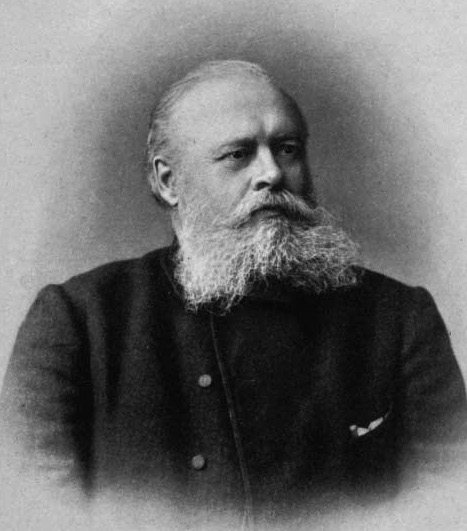
\includegraphics[width=\linewidth]{images/book2/markovnikov.jpg}
\end{minipage}\hfill
\begin{minipage}[t]{0.76\linewidth}\vspace{0pt}
Vladimir Markovnikov stated his rule in the nineteenth century, from the
products he and others observed, long before \omterm{def:b1:electronic-effects:intermediates}{carbocations} or \omterm{def:b1:electronic-effects:curly-arrow}{curly arrows}
existed: a regularity of nature, written down before it could be
explained. Its modern statement through \omterm{def:b1:electronic-effects:intermediates}{carbocation} stability shows what
a mechanism adds to an empirical rule: it says when the rule should fail.
(Portrait from an obituary notice published in 1905, public domain,
Wikimedia Commons.)
\end{minipage}
\end{history}

\section{Exercises}

\begin{exercise}[$\star$]\label{exo:b1:electrophilic-additions:1}
Give the main product of: propene + HCl; 2-methylpropene + HBr;
1-methylcyclohexene + HBr; but-2-yne + one equivalent of HCl.
\end{exercise}

\begin{exercise}[$\star$]\label{exo:b1:electrophilic-additions:2}
Write the products of bromine with ethene, cyclohexene and propene. Name
them.
\end{exercise}

\begin{exercise}[$\star$]\label{exo:b1:electrophilic-additions:3}
Which alcohol does the acid-catalysed \omterm{def:b1:electrophilic-additions:hydration}{hydration} of each alkene give:
propene, 2-methylpropene, methylenecyclohexane?
\end{exercise}

\begin{exercise}[$\star$]\label{exo:b1:electrophilic-additions:4}
Which of these compounds react with sodium amide: propyne, but-2-yne,
propene, ethanol? Write the reactions.
\end{exercise}

\begin{exercise}[$\star\star$]\label{exo:b1:electrophilic-additions:5}
Write the full mechanism of the \omterm{def:b1:electrophilic-additions:hydration}{hydration} of 2-methylpropene with \omterm{def:b1:electronic-effects:curly-arrow}{curly
arrows}, and explain why the reverse reaction is favoured in hot
concentrated acid.
\end{exercise}

\begin{exercise}[$\star\star$]\label{exo:b1:electrophilic-additions:6}
Explain with the Hammond postulate why 2-methylpropene reacts with HCl
much faster than propene.
\end{exercise}

\begin{exercise}[$\star\star$]\label{exo:b1:electrophilic-additions:7}
Bromine reacts with cyclohexene. Show that the product is
\textit{trans}-1,2-dibromocyclohexane, and say whether it is \omterm{def:b1:stereochemistry-in-depth:stereocentre}{chiral} and
whether the product is optically active.
\end{exercise}

\begin{exercise}[$\star\star$]\label{exo:b1:electrophilic-additions:8}
Propose a mechanism for the addition of HCl to 3-methylbut-1-ene that
gives mainly 2-chloro-2-methylbutane.
\end{exercise}

\begin{exercise}[$\star\star$]\label{exo:b1:electrophilic-additions:9}
Propose a synthesis of hex-2-yne from propyne and a halogenoalkane, and
of 1-phenylbut-2-yn-1-ol from propyne and benzaldehyde.
\end{exercise}

\begin{exercise}[$\star\star\star$]\label{exo:b1:electrophilic-additions:10}
Prove the stereochemistry of bromine addition to the two but-2-enes by
drawing: bromonium ion, anti attack at each carbon, \omterm{def:b1:stereochemistry-in-depth:representations}{Cram representation}
of the products, descriptors. Count the \omterm{def:b1:stereochemistry-in-depth:isomers}{stereoisomers} formed in each
case.
\end{exercise}

\begin{exercise}[$\star\star\star$]\label{exo:b1:electrophilic-additions:11}
Bromine water with propene gives 1-bromopropan-2-ol as the main product.
Explain the regiochemistry: why does water attack the more substituted
carbon of the bromonium ion?
\end{exercise}

\begin{exercise}[$\star\star\star$]\label{exo:b1:electrophilic-additions:12}
A hydrocarbon \ce{C5H10} decolourises bromine water and adds HBr to give
2-bromo-2-methylbutane; its \omterm{def:b1:electrophilic-additions:hydration}{hydration} gives 2-methylbutan-2-ol. Find two
possible structures and propose a way to tell them apart.
\end{exercise}

\section{Problem: Two Butenes and Bromine}

\begin{problem}[{Weekend problem --- the two but-2-enes, the bromonium
mechanism, meso and racemic dibromides, their optical rotation and the
mass obtained}]
\label{pb:b1:electrophilic-additions:1}
A laboratory has two bottles of but-2-ene, one pure \cip{Z}, one pure
\cip{E}, and treats \qty{5.60}{g} of each with bromine in
dichloromethane. Molar masses (\unit{g/mol}): \ce{C4H8} 56.0, \ce{Br2}
159.8, \ce{C4H8Br2} 215.8.

\medskip
\noindent\textbf{Part I --- The two alkenes.}
\begin{enumerate}
  \item Draw \cip{Z}- and \cip{E}-but-2-ene and justify the descriptors.
  \item Are they \omterm{def:b1:stereochemistry-in-depth:isomers}{stereoisomers}? \omterm{def:b1:stereochemistry-in-depth:enantiomers}{Enantiomers} or \omterm{def:b1:stereochemistry-in-depth:enantiomers}{diastereomers}?
  \item Why do they not interconvert at room temperature?
  \item Which is the more stable, and why?
  \item Write the overall equation of the addition of bromine.
  \item How many stereocentres has 2,3-dibromobutane? How many
        \omterm{def:b1:stereochemistry-in-depth:isomers}{stereoisomers} at most, and how many in fact?
\end{enumerate}

\medskip
\noindent\textbf{Part II --- The mechanism.}
\begin{enumerate}[resume]
  \item Write the formation of the bromonium ion with \omterm{def:b1:electronic-effects:curly-arrow}{curly arrows}.
  \item Why is a bridged bromonium ion formed rather than an open
        \omterm{def:b1:electronic-effects:intermediates}{carbocation}?
  \item Write the opening of the ion by bromide.
  \item Why does bromide attack from the face opposite the bridge?
  \item What kind of addition results?
  \item Why is the solvent dichloromethane and not water?
\end{enumerate}

\medskip
\noindent\textbf{Part III --- The products.}
\begin{enumerate}[resume]
  \item From \cip{E}-but-2-ene: draw the product of attack at C2 and give
        the descriptors of C2 and C3.
  \item Same for attack at C3. Compare.
  \item Show that the product is meso.
  \item From \cip{Z}-but-2-ene: draw the two products and their
        descriptors.
  \item In what proportions are they formed? Name the mixture.
  \item Is the reaction stereospecific? Justify.
\end{enumerate}

\medskip
\noindent\textbf{Part IV --- Rotation and mass.}
\begin{enumerate}[resume]
  \item What optical rotation does the product of the \cip{Z} alkene show?
  \item Compute the amount of each alkene.
  \item Compute the mass of dibromide expected from each at
        \qty{85}{\percent} \omterm{def:b1:extent-q-and-k:fractional-extent}{yield}.
  \item State the \omterm{def:b1:stereochemistry-in-depth:optical-activity}{specific rotation} of the dibromide obtained from
        \cip{E}-but-2-ene, and the mass of it obtained.
\end{enumerate}
\end{problem}
